\documentclass[spanish]{report} % article, book

\usepackage[spanish]{babel} % idioma castellano
\usepackage{graphicx} % imágenes
\usepackage{hyperref} % links


\setlength{\parindent}{0cm} % sin sangría
\renewcommand\thesection{\arabic{section}}
\renewcommand\thesubsection{\arabic{subsection}}

\title{Redes y Aplicaciones Internet - Práctica 1}
\author{Oussama Akachach Jouhrati} % Oussama Akachach Jouhrati\\[]{\small Profesor/a: }
\date{\today}

\hypersetup {
        linktoc=all,
        hidelinks
}

\begin{document}

\maketitle
\tableofcontents
\setcounter{page}{2}

\begin{abstract}

En esta práctica se han realizado tres actividades relacionadas con el anális del
tráfico de la red mediante el software Wireshark. Tras haber instalado el
programa y preparado la herramienta, hemos analizado la web edu4java.com, donde
hemos capturado tramas que posteriormente se han utilizado para resolver las
preguntas planteadas por el/la profesor/a.\newline

Estas actividades han consistido en análisis de los diferentes protocolos
utilizados por los paquetes enviados y recibidos tras interactuar con la página
mencionada anteriormente, en los diferentes niveles del proceso (enlace, red,
transporte y aplicación).\newline

Cada una de estas actividades se ha realizado mediante la lectura previa de los
contenidos del libro \textit{Computer Networking. A Top-Down Approach}, de James
F. Kurose y Keith W. Ross. Estas se tenían que hacer secuencialmente y se
conseguía una nota mínima más alta por cada actividad resuelta correctamente.

\end{abstract}

\setcounter{page}{3}

\section{Parte 1. El nivel de enlace y de red}

\subsection{Pregunta 1}

\begin{figure}[h]
\begin{center}
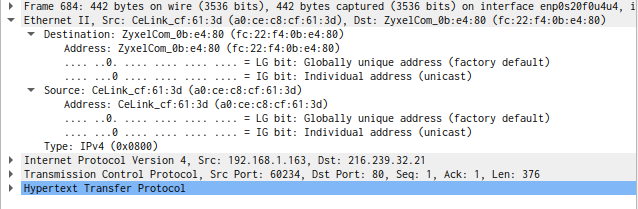
\includegraphics[scale=.5]{../img/1.png}
\end{center}
\caption{Captura de pantalla de la cabecera Ethernet con datos de la capa de
enlace}
\end{figure}

\subsubsection{Apartado a}
La dirección origen es: \textbf{a0:ce:c8:cf:61:3d}.\newline

La dirección destino es: \textbf{fc:22:f4:0b:e4:80}.

\subsubsection{Apartado b}
El fabricante asigna la dirección MAC de cada dispositivo.

\subsubsection{Apartado c}
El campo tipo nos indica la clase de protocolo de red que estamos utilizando
para transmitir los datos. Este puede ser de tipo IP, pero existen otros,
dependiendo de los que soporte el host.


\subsubsection{Apartado d}
El objetivo del campo CRC es permitir que el destinatario pueda detectar errores
de bit en la capa.


\subsubsection{Apartado e}
El campo preámbulo sirve para ``despertar'' los adaptadores del destinatario y
sincronizar su reloj al del remitente.


\subsubsection{Apartado f}

fc 22 f4 0b e4 80 a0 ce c8 cf 61 3d 08 00\newline

\begin{enumerate}
\item La dirección MAC del destinatario (fc 22 f4 0b e4 80)
\item La dirección MAC de la fuente (a0 ce c8 cf 61 3d)
\item El tipo de protocolo (08 00). En este caso, IPv4.
\end{enumerate}
La trama Ethernet lleva una datagrama IP.

Captura de pantalla de la cabecera Ethernet con datos de la capa de
enlace
\subsection{Pregunta 2}

\begin{figure}[h]
\begin{center}
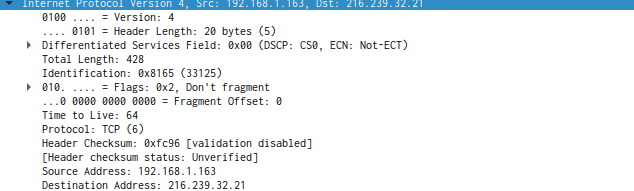
\includegraphics[scale=.5]{../img/2.png}
\end{center}
\caption{Captura de pantalla de la cabecera IP}
\end{figure}

\subsubsection{Apartado a}
La dirección IP origen es 192.168.1.163 y corresponde a la dirección IP de mi
router.\newline

La dirección IP destino es 216.239.32.21 y corresponde a la dirección IP de la
página edu4java.

\subsubsection{Apartado b}
Cuando un datagrama IP es demasiado largo como para enviarse en un solo paquete,
este se fragmenta en múltiples paquetes. Este identificador nos permite
reconstruir más adelante el datagrama completo.

\subsubsection{Apartado c}
El flag activo en este paquete es 0x2.

\subsubsection{Apartado d}
El campo TTL (time to live) sirve para que los datagramas no circulen
eternamente en la red. Por cada vez que este datagrama sea procesado por
unrouter, el valor decrecerá en una unidadm hasta llegar a cero, donde se deberá
descartar dicho datagrama.\newline

En este caso, a nuestro paquete le quedan todavía 64 interacciones con un
router, para ser descartado.

\subsubsection{Apartado e}
El campo Header Checksum nos sirve para detectar errores en la transmisión de
datos en la capa IP. Este proceso se debe volver a hacer puesto que el campo de
opciones y el campo TTL puede cambiar y debemos asegurarnos de que el checksum
que llevamos sea el mismo que el computado.

\subsubsection{Apartado f}
Se han enviado más paquetes con el protocolo TCP, siendo en total 676 paquetes,
representando un 78.15 por ciento. El resto ha sido mediante el protocolo UDP,
siendo 189 paquetes o un 21.85 por ciento.\newline

La razón consiste en que, al conectarnos a la página, hemos realizado conexiones
a un servidor pasivo que estaba a la espera de clientes que se conectaran. TCP
se trata de un protocolo orientado a conexiones, mientras que UDP está enfocado
a mensajes y se trata de un protocolo que no depende de conexiones.

\subsection{Pregunta 3}

\begin{figure}[h]
\begin{center}
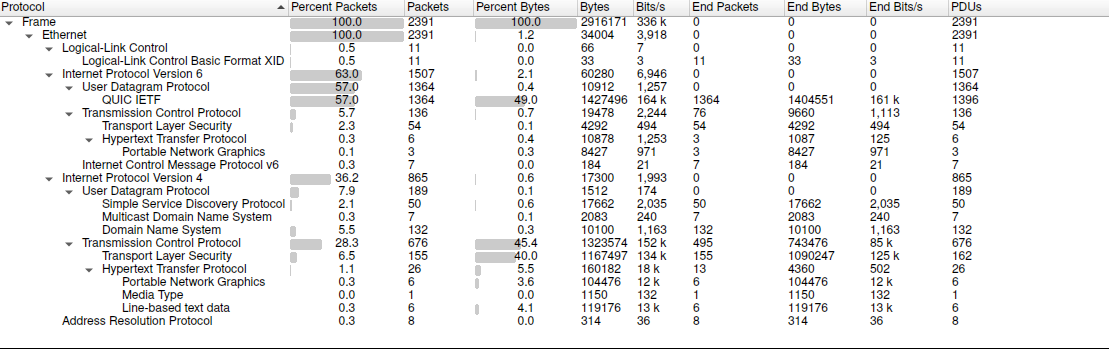
\includegraphics[scale=.3]{../img/3.png}
\end{center}
\caption{Captura de pantalla de la pantalla Statistics/Protocol Hierarchy}
\end{figure}

\newpage

Para empezar, podemos ver que todos los paquetes han sido enviados a través de
una interfaz Ethernet. Esto es debido a que el ordenador sobre el cual se está
realizando el análisis está conectado a través de una conexión por
cable.\newline

Seguido de ello, vemos que los dos tipos de protocolos que se han usado han sido
IPv6 e IPv4, donde IPv6 ha sido el que más paquetes ha movido, de los cuales el
protocolo con más paquetes ha sido UDP, seguido de TCP. Esto es debido a que
encima de UDP, tenemos QUIC, que es un tipo de protocolo de red de la capa de
transporte utilizado por aproximadamente el 30 por ciento del tráfico de red en
2021. Lo maś probable es que estemos utilizando este método para conectarnos al
backend de la página, donde el servidor de ésta debe utilizar este tipo de
protocolo.\newline

Dentro de los paquetes enviados con IPv4, vemos que la mayoría han sido TCP, en
este caso, concretamente han sido a través de HTTP, puesto que al conectarnos a
la página, hemos realizado requests para obtener el contenido de dicha, de los
cuales tenemos 6 paquetes para png's, 1 de Media Types y 6 de datos de texto,
que puede ser el propio html de la página.


\newpage
\section{Parte 2. El nivel de transporte}

\subsection{Pregunta 1}

\begin{figure}[h]
\begin{center}
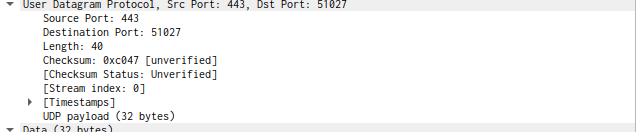
\includegraphics[scale=.5]{../img/4.png}
\end{center}
\caption{Captura de pantalla de la capa de transporte de un paquete con
protocolo UDP}
\end{figure}

\subsubsection{Apartado a}
Estos paquetes han generado protocolos de tipo Data, en los que tenemos una
cadena de caracteres de longitud variable, según el paquete.

\subsubsection{Apartado b}
En caso de partir con mecanismos de reconocimiento y retransmisión en la propia
aplicación, podemos aprovecharnos de la velocidad del protocolo UDP, ya que TCP
tiene limitaciones en su velocidad de transmisión por sus mecanismos de control
de congestiones.

\subsubsection{Apartado c}
El puerto origen es 443 y el puerto destino es 51027. Significa que este número
permitirá que el host de destino pase los datos de la aplicación al correcto
proceso para su interpretación.


\subsubsection{Apartado d}
El campo checksum es necesario para que el remitente pueda verificar si se han
introducido errores en el segmento.


\subsubsection{Apartado e}
Se hace la suma de todas las palabras de 16 bits y se calcula el complementario
del resultado, donde los unos se convierten a ceros y los ceros, a unos. El
resultado de esta operación será el checksum.\newline

Cuando termine la operación de transmisión, al destinatario le llegará la suma
de todas las palabras, más el valor del checksum. Si la suma de todo da todo
unos, entonces no se han producido errores, pero con que haya un cero, sabemos
que ha ocurrido algo no esperado.

\subsubsection{Apartado f}
En el campo Length tenemos el valor 40. Esto se puede comprobar contando todos
los bytes de la cadena hexadecimal, desde el comienzo de la capa de transporte,
hasta el final del datagrama.\newline

Bytes de la capa de transporte: 01 bb c7 53 00 28 c0 47 (8 bytes)\newline

Bytes de la capa de aplicación: 55 86 3e 95 78 08 fe 4d 69 9c 48 d4 86 95 25 ab
0010   a9 b5 c1 08 55 73 2f e0 c7 35 6f e4 ee 69 3f cd (32 bytes)\newline

Si hacemos la suma (8 + 32), el resultado da 40, correspondiéndose con el campo
Length.

\subsection{Pregunta 2}

\begin{figure}[h]
\begin{center}
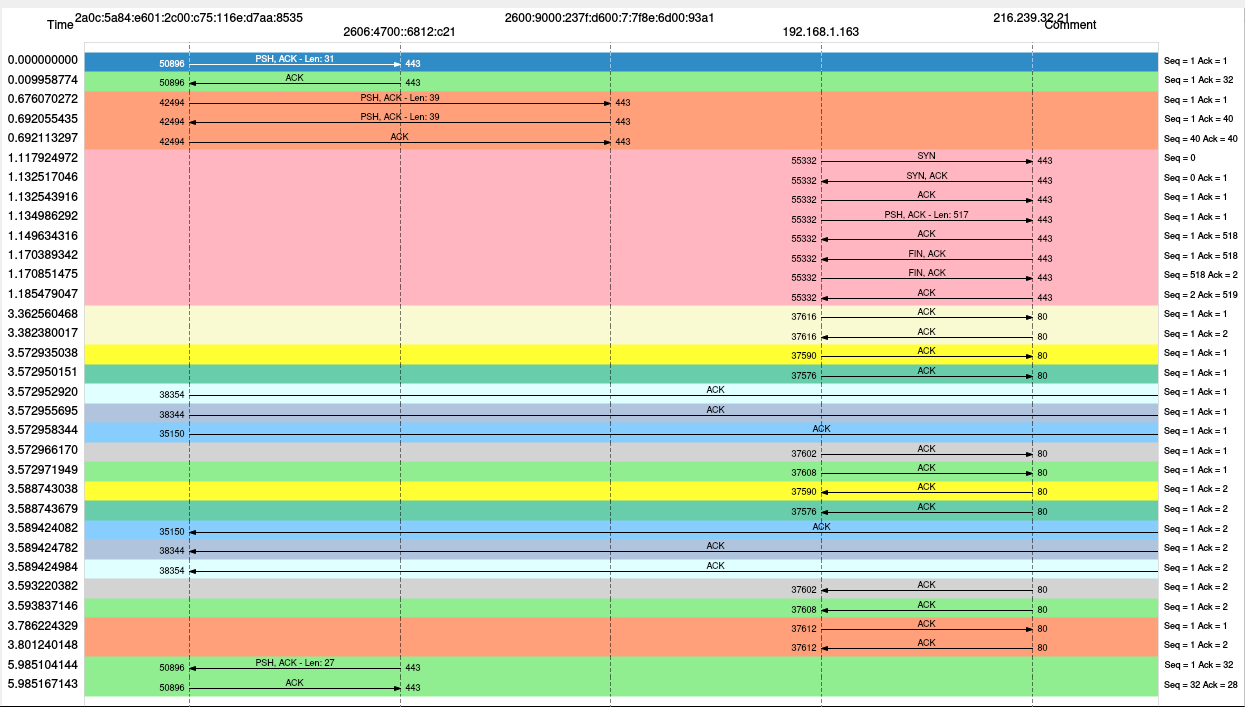
\includegraphics[scale=.25]{../img/6.png}
\end{center}
\caption{Diagrama de flujo con filtro TCP}
\end{figure}

En el timestamp 1.11, el flag SYN nos indica que se está configurando la
conexión y, por lo tanto, su establecimiento. El siguiente paquete enviado tras
este viene de vuelta del destinatario, conforme se ha realizado la operación
correctamente y se ha establecido una conexión.\newline

Más adelante, se envía un paquete de longitud 517 bytes, y en el siguiente
paquete de vuelta, el destinatario nos devuelve un ACK con un valor de 518,
indicando que ha recibido correctamente los 517 bytes y está a la espera de los
siguientes. Un proceso similar aparece en los siguientes paquetes, donde
se utiliza el flag FIN, utilizado también para establecer
conexiones.\newline

Más adelante, se cambia al puerto 80 del destinatario, donde antes era 443, y
se envían más paquetes con un flag ACK igual a 1. El destinatario
devuelve la información al remitente con un ACK igual a 2, indicando que ha
recibido ese primer byte y está a la espera de recibir los
siguientes.\newline

Sabemos que ese tráfico corresponde a la conexión con la página porque las
direcciones IP marcadas en la parte superior del gráfico corresponden a la
IP del router del remitente y a la de la página del destinatario,
respectivamente.\newline

El flag PSH indica al destinatario que debe pasar los datos a las capas
superiores inmediatamente.

\subsection{Pregunta 3}

\begin{figure}[h]
\begin{center}
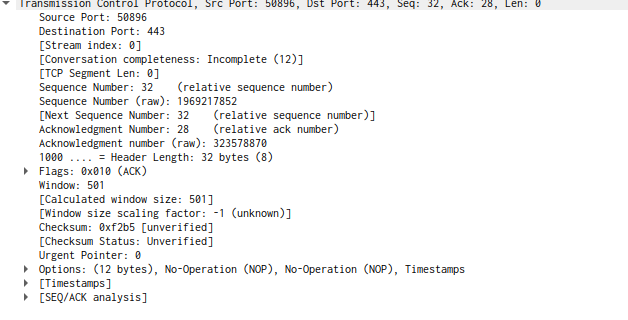
\includegraphics[scale=.5]{../img/5.png}
\end{center}
\caption{Captura de pantalla de la capa de transporte de un paquete con
protocolo TCP}
\end{figure}


\subsubsection{Apartado a}
El número de secuencia es 32. Se utiliza por el remitente en TCP para
implementar un servicio de transferencia de datos fiable.

\subsubsection{Apartado b}
El número de ACK es 1. Se utiliza para indicar que el valor almacenado en el
campo de reconocimiento es válido. Con esto queremos decir que el segmento
contiene un reconocimiento de un segmento que ya ha sido recibido con éxito.

\subsubsection{Apartado c}
El puerto origen tiene un valor de 50896 y el puerto destino tiene un valor de
443. Se utilizan de una manera similar al protocolo UDP, para que las
aplicaciones de capas más elevadas puedan destinar la información a los lugares
donde se procesen debidamente.

\subsubsection{Apartado d}
En este paquete tenemos únicamente el flag ACK, con un valor de 0x010.

\subsubsection{Apartado e}
Se utiliza para el control del flujo y para indicar el número de bytes que un
destinatario está dispuesto a aceptar.

\subsubsection{Apartado f}
Tiene 12 bytes en el apartado de opciones. Dentro de este apartado, tenemos dos
opciones de tipo No-Operation (NOP) y una opción Timestamps, de 10 bytes de
longitud, en la que se indica el tipo de opción, la longitud, el valor del
timestamp y el valor de respuesta del timestamp de vuelta.


\newpage
\section{Parte 3. El nivel de aplicación}

\subsection{Pregunta 1}

\begin{figure}[h]
\begin{center}
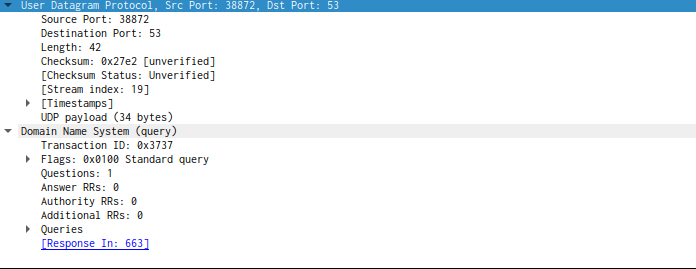
\includegraphics[scale=.5]{../img/7.png}
\end{center}
\caption{Captura de pantalla de la cabecera DNS de una petición}
\end{figure}

\begin{figure}[h]
\begin{center}
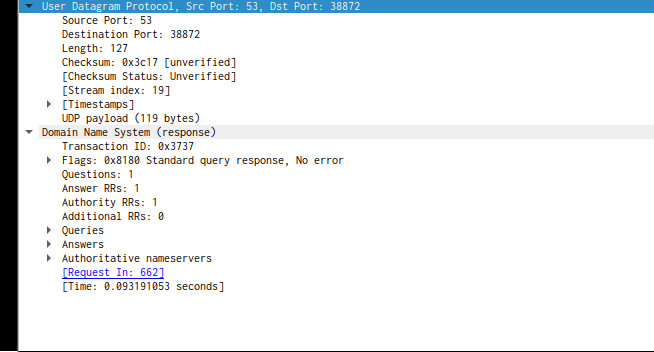
\includegraphics[scale=.5]{../img/8.png}
\end{center}
\caption{Captura de pantalla de la cabecera DNS de una respuesta}
\end{figure}

\newpage

\subsubsection{Apartado a}

En la petición, los puertos origen y destino son 38872 y 53,
respectivamente.\newline

En la respuesta, los puertos origen y destino se intercambian, siendo 53 y
38872, respectivamente.

\subsubsection{Apartado b}

Para poder relacionar los paquetes de petición y respuesta entre todo el listado
de paquetes.

\subsubsection{Apartado c}

Sirven para poder identificar el tipo de paquete. En el caso de las Standard
query, utilizamos el flag 0x0100, mientras que para las Standard query response
utilizamos el flag 0x8180.

\subsubsection{Apartado d}

En la petición se está preguntando por el dominio www.edu4java.com.

\subsubsection{Apartado e}

Este dominio es de tipo AAAA y su clase es de tipo IN.\newline

Que el dominio sea de tipo A significa que el campo Name es un hostname y el
campo Value es la dirección IP del hostname. Además, el mapeo del registro
sigue la siguiente estructura: hostname, dirección IP, tipo.\newline

Que la clase sea de tipo IN hace referencia a ``Internet''. La única opción
alternativa sería CH, para ``Chaos''. Mientras que la clase CH se utiliza para
consultar versiones de servidores DNS, la clase IN se utiliza para acciones más
generales de Internet. 

\subsubsection{Apartado f}

Sí, cada mensaje de respuesta del DNS transporta uno o más RRs. En este caso,
tenemos uno para la consulta, otro para las respuestas y otro de autoridad.

\newpage

\subsection{Pregunta 2}

\begin{figure}[h]
\begin{center}
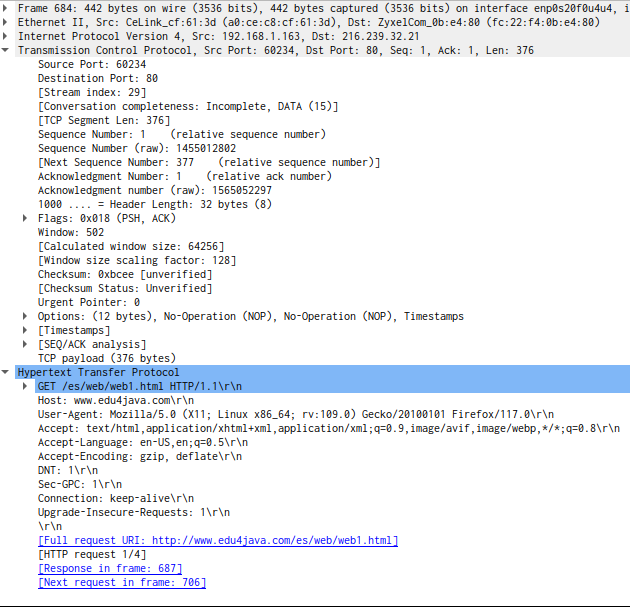
\includegraphics[scale=.4]{../img/9.png}
\end{center}
\caption{Captura de pantalla de la cabecera HTTP de una petición GET}
\end{figure}

\subsubsection{Apartado a}

Se utilizan los puertos origen y destino 60234 y 80, respectivamente.

\subsubsection{Apartado b}

Se utiliza la versión 1.1 del protocolo HTTP.

\subsubsection{Apartado c}

No, es una conexión que se cierra una vez hemos recibido el objeto solicitado,
en este caso, el objeto /es/web/web1.html.

\subsubsection{Apartado d}

Se utiliza el idioma en-US o inglés de Estados Unidos. Se facilita para que, en
caso de que la página tenga una versión de la página para nuestra preferencia de
idioma, se nos facilite esta en lugar de la predeterminada.

\subsubsection{Apartado e}

Esta petición acepta los siguientes tipos de datos:

\begin{enumerate}

\item text/html

\item application/xhtml+xml

\item application/xml

\item image/avif

\item image/webp

\end{enumerate}

\subsubsection{Apartado f}

Esta petición acepta los siguientes formatos de codificación: gzip y deflate.
\subsection{Pregunta 3}

\begin{figure}[h]
\begin{center}
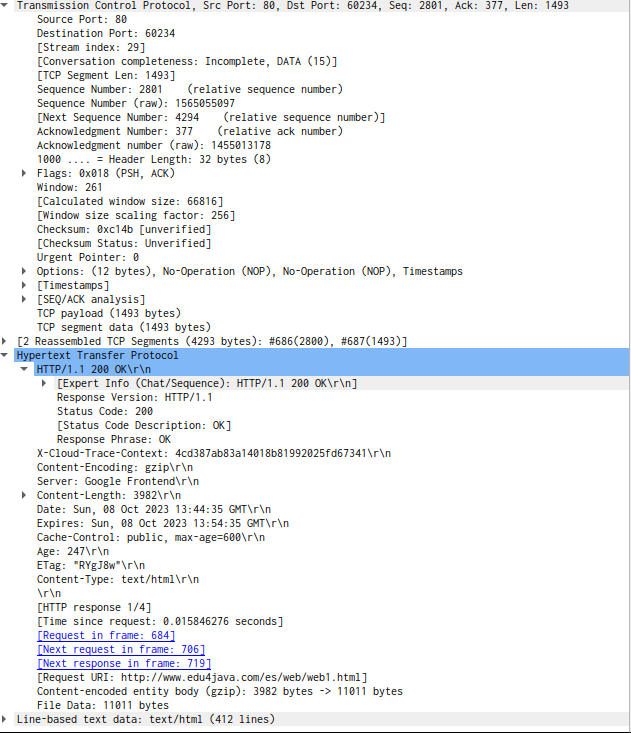
\includegraphics[scale=.35]{../img/10.png}
\end{center}
\caption{Captura de pantalla de la cabecera DNS de una petición}
\end{figure}


\subsubsection{Apartado a}

Esta respuesta contiene un mensaje de tipo 200 OK y un objeto de respuesta.

\subsubsection{Apartado b}

Se trata de un contenido de tipo text/html, correspondiente a la página web de
edu4java que visitamos.

\subsubsection{Apartado c}

Sí, esto lo podemos saber ya que en el apartado [HTTP response 1/4] nos está
informando de que este paquete es una respuesta de cuatro totales para
satisfacer la primera petición.\newline

También lo podemos saber mediante el campo Content-encoded entity body (gzip),
donde nos informa que nos han llegado 3982 bytes de un total de 11011.

\subsubsection{Apartado d}

Tenemos el campo Date, que corresponde la fecha a la que se ha enviado el objeto
del servidor al cliente y el campo Expires, que es el momento de timeout, donde
se asume que no se ha realizado una conexión exitosa tras no recibir respuesta.

\subsubsection{Apartado e}

Sí, el campo X-Cloud-Trace-Context se trata de un identificador de cookie
utilizado por la página. Estas sirven para registrar la actividad del cliente y
poder añadir personalización a una página estática.\newline

Esta funcionalidad sirve para que el servidor recuerde la actividad del
navegador que utilizamos, asociándola al identificador mencionado.

\subsubsection{Apartado f}

Los campos relacionados con cachés sirven para que, en caso de que nuestro
cliente ya tenga una versión del objeto a consultar, este realice la consulta a
sus propios archivos, en lugar de solicitarlo al servidor. De esta manera, se
ahorra ancho de banda para ambos lados.

\newpage

\subsection{Pregunta 4}

\begin{figure}[h]
\begin{center}
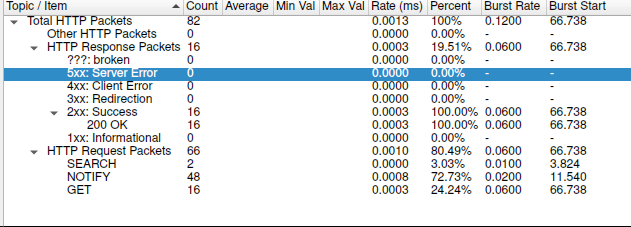
\includegraphics[scale=.5]{../img/11.png}
\end{center}
\caption{Captura de pantalla del packet counter de Statistics/HTTP}
\end{figure}

Esta sesión no ha tenido ninguna respuesta no exitosa. Esto se puede ver por el
tipo de mensaje de respuesta. Todas las respuestas HTTP (16) han sido de tipo
2xx, que sirven para indicar éxitos. Concretamente, estas han sido de
tipo 200, que indican que la petición ha sido respondida correctamente.\newline

En caso de que hubiesen habido errores, serían del tipo 4xx para errores del
lado del cliente, y del tipo 5xx para errores del lado del servidor. Los
mensajes de tipo 3xx son redirecciones. De todos estos tipos, no hemos recibido
ninguna respuesta.\newline

En caso de haber tenido un error del lado de cliente, por ejemplo, al introducir
una URL incorrecta en una petición GET, nos hubiese llegado un error 404 NOT
FOUND, conforme no ha encontrado el objeto que solictábamos.\newline

En caso de que el servidor estuviese caído, nos hubiese devuelto una petición de
tipo 500 INTERNAL SERVER ERROR, donde el servidor no ha podido dar respuesta a
nuestra petición por motivos ajenos al cliente, como por ejemplo, un
NullPointerException a la hora de interactuar con el backend para devolver los
datos.\newline

Al no haber tenido ningún mensaje de error, se describen dos escenarios bastante
comunes de respuestas fallidas y sus códigos de error respectivos.

\newpage
\section{Parte 4. Seguridad en la red}

\subsection{Pregunta 1}

\begin{figure}[h]
\begin{center}
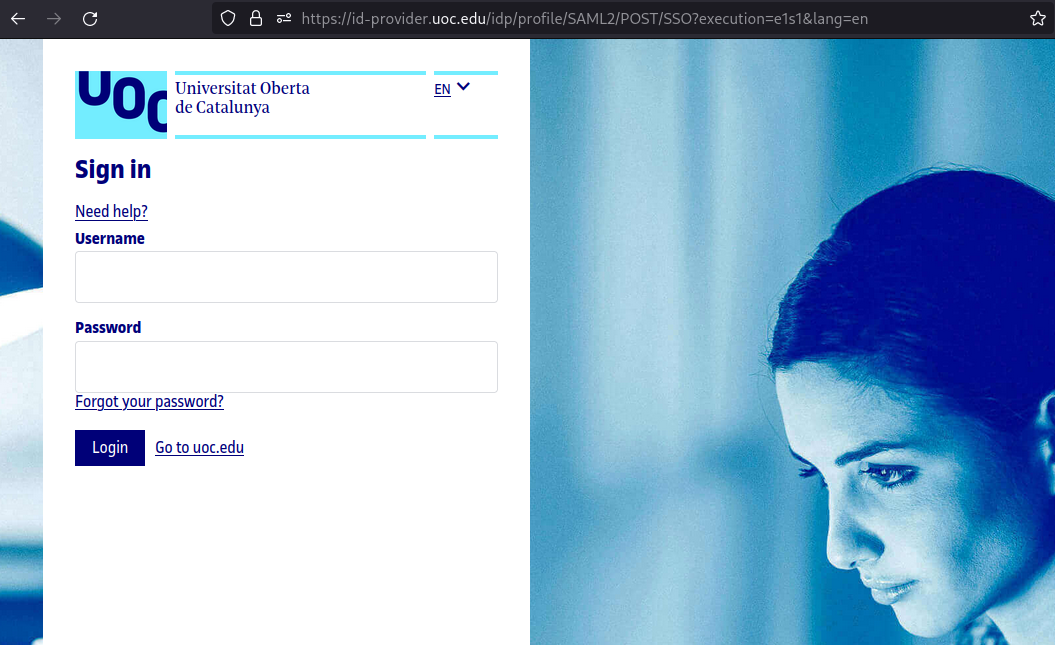
\includegraphics[scale=.3]{../img/12.png}
\end{center}
\caption{Captura de pantalla de la página de inicio de sesión del Campus}
\end{figure}

\subsection{Pregunta 2}

En el nivel de aplicación se utiliza el protocolo DNS para acceder al Campus
Virtual de la UOC. Este protocolo se caracteriza por servir de traductor entre
el nombre de un dominio, por ejemplo aula.uoc.edu, a una dirección IP, que es lo
que realmente se necesita para acceder a una página.

\newpage

\subsection{Pregunta 3}

\begin{figure}[h]
\begin{center}
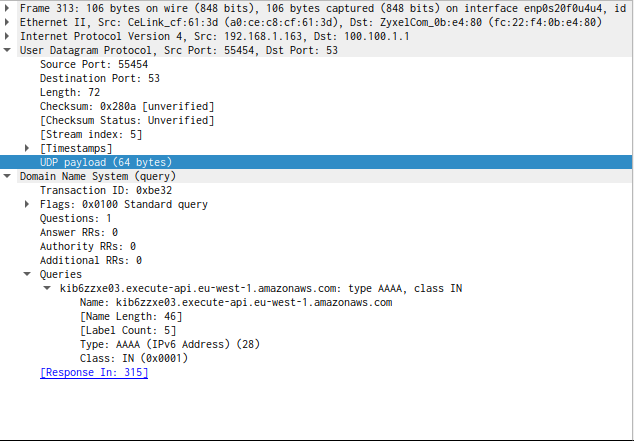
\includegraphics[scale=.5]{../img/13.png}
\end{center}
\caption{Captura de pantalla de un paquete concreto de este protocolo}
\end{figure}

Este paquete utiliza el protocolo DNS como protocolo en el nivel de aplicación.
Se trata de una consulta DNS y tiene el ID de transacciń 0xbe32. Este nos
servirá para poder enlazar esta petición con la respuesta que nos devuelva el
servidor.\newline

Tiene un único flag, de valor 0x0100, representado mediante el nombre de
Standard Query, al ser una consulta normal. Además, tiene un número RR, de tipo
Pregunta y la consulta que se realiza es al dominio
kib6zzxe03.execute-api.eu-west-1.amazonaws.com, de tipo A y de clase IN. Con
esto sabemos que nos estamos conectando a servidores de AWS para realizar la
conexión al Campus Virtual y que se trata de una conexión hecha a través de
Internet, por la clase IN.

\subsection{Pregunta 4}

El protocolo DNS utiliza UDP como protocolo de nivel de transporte.
\newpage

\subsection{Pregunta 5}

\begin{figure}[h]
\begin{center}
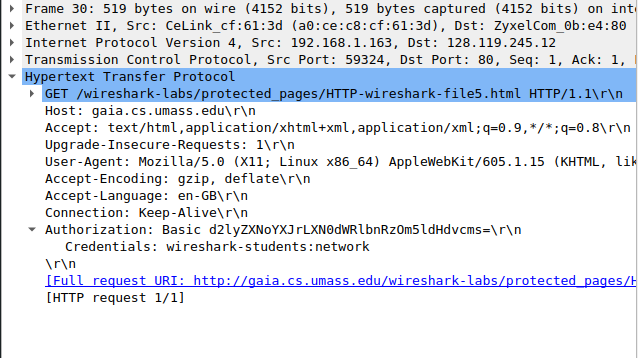
\includegraphics[scale=.5]{../img/14.png}
\end{center}
\caption{Captura de pantalla de la cabecera HTTP después de la autenticación}
\end{figure}

\begin{thebibliography}{X}

\item Awati, R. (2022). Persistent connection. WhatIs.com.
https://www.techtarget.com/whatis/definition/persistent-connection-HTTP-persistent-connection

\item Differences between TCP and UDP. (2022, April 18). Spiceworks.
https://www.spiceworks.com/tech/networking/articles/tcp-vs-udp/

\item Eastlake, R. D., Brunner-Williams, E., \& Manning, B. (2000b). Domain Name
System (DNS) IANA Considerations. https://doi.org/10.17487/rfc2929

\item IONOS editorial team. (2023). MAC address (media access control). IONOS
Digital Guide. https://www.ionos.com/digitalguide/server/know-how/mac-address/

\item Kurose, J. F., Ross, K. W. (2021). \textit{Computer networking: A Top-down
Approach}

\end{thebibliography}

\end{document}


% center

% \begin{center} \end{center}

% tables

% \begin{tabular} text \\ \hline \end{tabular}

% abstract

% \vspace{0.5cm} espacio artificial


